% ****** Start of file apssamp.tex ******
%
%   This file is part of the APS files in the REVTeX 4.2 distribution.
%   Version 4.2a of REVTeX, December 2014
%
%   Copyright (c) 2014 The American Physical Society.
%
%   See the REVTeX 4 README file for restrictions and more information.
%
% TeX'ing this file requires that you have AMS-LaTeX 2.0 installed
% as well as the rest of the prerequisites for REVTeX 4.2
%
% See the REVTeX 4 README file
% It also requires running BibTeX. The commands are as follows:
%
%  1)  latex apssamp.tex
%  2)  bibtex apssamp
%  3)  latex apssamp.tex
%  4)  latex apssamp.tex
%
\documentclass[%
 reprint,
%superscriptaddress,
%groupedaddress,
%unsortedaddress,
%runinaddress,
%frontmatterverbose, 
%preprint,
%preprintnumbers,
%nofootinbib,
%nobibnotes,
%bibnotes,
 amsmath,amssymb,
 aps,
%pra,
%prb,
%rmp,
%prstab,
%prstper,
%floatfix,
]{revtex4-2}

\usepackage{graphicx}% Include figure files
\usepackage{dcolumn}% Align table columns on decimal point
\usepackage{esvect}% custom arrow styles
\usepackage{bm}% bold math
\usepackage{algorithm}
\usepackage{algpseudocode}
%\usepackage{hyperref}% add hypertext capabilities
%\usepackage[mathlines]{lineno}% Enable numbering of text and display math
%\linenumbers\relax % Commence numbering lines

%\usepackage[showframe,%Uncomment any one of the following lines to test 
%%scale=0.7, marginratio={1:1, 2:3}, ignoreall,% default settings
%%text={7in,10in},centering,
%%margin=1.5in,
%%total={6.5in,8.75in}, top=1.2in, left=0.9in, includefoot,
%%height=10in,a5paper,hmargin={3cm,0.8in},
%]{geometry}

\usepackage[dvipsnames]{xcolor}
\definecolor{roie}{rgb}{0.858, 0.188, 0.478}

\begin{document}

\preprint{APS/???}

\title{Learning Network}

\author{Roie Ezraty}
 \email{roie.ezraty@mail.huji.ac.il}
\author{Shmuel M. Rubinstein}%
\affiliation{Racah Institute of Physics, Hebrew University of Jerusalem, Jerusalem 9190401, Israel
}

\date{\today}% It is always \today, today,
             %  but any date may be explicitly specified

\maketitle

\begin{abstract}

Abstract - 

\end{abstract}

\section{Introduction}\label{sec:Introduction}

    1) We often want to make a physical material perform a desired task, as in folding a protein to produce certain functionality \textcolot{roie}{(cite)} or reducing the flow obstruction in a flow network \textcolot{roie}{(cite)}. We often have only minimal access to change the material's internal degrees of freedom, lack a-priori knowledge of the task itself before setting up the material or knowledge of its internal state as it functions. 
    Over the last decades, a substitution was set-up, as external processors such as computers have been a major player in the field of task performance. These have both the ability to learn multiple tasks while providing access to all degrees of freedom and the ability to perform calculations that are global, using information from all the processing units, which is often infeasible in physical systems. 
    Still, there is great endeavor in finding out how physical systems can be harnessed instead \cite{lopez2023self}. 
    Firstly, computation on an external processor requires converting a task into digital signal, doing calculations in the digital world and then converting it back to the desired medium to get the desired functionality, whereas in a physical system the calculation and functionality can be encompassed in the same medium \cite{stern2023learning}. 
    Secondly, global calculation is rather costly, especially during the backpropagation procedure \cite{xie2003equivalence}, whereas  a physical system obeying local rules could render the calculation much more scalable and efficient.
    Thirdly, gradient-descent and backpropagation calculated on the external processor require energy and do not attempt to spend it efficiently, leading to large power expenditure for training machines \cite{luccioni2023estimating, mytton2022sources} whereas physical systems that minimize power dissipation strive to be power efficient inherently \cite{berneman2024designing}.
    Nature itself testifies on this notion; Learning systems that use only local information are still versatile to a variety of tasks, \textcolor{roie}{are robust against damage, and learn in very short time scales.}

    2) Physical materials that minimize power dissipation can be trained using "directed-aging", where the material (be it mechanical networks, flow networks, etc.) is strained to a desired functionality \cite{pashine2019directed, hexner2020effect}. This learning scheme capitalizes on local evolution rules in the material without the information on the internal degrees of freedom in the system. It is, however, limited in the scope of tasks that can be performed.

    3) More versatile training schemes, termed "contrastive learning" \cite{scellier2017equilibrium}, or its more physical counterpart "coupled learning" \cite{stern2021supervised}, that comply with "equilibrium propagation" \cite{scellier2021deeplearningtheoryneural} in the limit of small changes to degrees of freedom, also capitalize on local physical rules, but have been shown to solve more stringent tasks than those demonstrated with directed aging \cite{dillavou2022demonstration, altman2024experimental}. 
    These are decentralized, physics-based learning systems that can be very efficient in terms of power dissipation \cite{stern2024training}, and \textcolor{roie}{???}. However, there is still the need to access internal parameters, which is sometimes not feasible in physical systems.

    4) Here, we develop a scheme where a system that minimizes power dissipation (e.g. a resistor network) is strained using only its inputs (e.g. pressures) \cite{gold2019self, kedia2019drive}. We only require that the internal degrees of freedom (e.g. resistors, also referred to as "learning" degrees of freedom \cite{dillavou2022demonstration}) have some dependence on the response of the system to the inputs. 
    First, an input is posed on the system and the output is measured. The internal degrees of freedom do not change but are also not observed. 
    A loss is calculated with respect to the desired output and then new values are posed on inputs and outputs. The system it responds to them by changing the internal degrees of freedom, without the user knowing their values at any time. 
    Since during measurement of the outputs the internal degrees of freedom do not change, they do so only when also outputs are constrained, we termed the scheme the "dual state" scheme. 
    Changes in internal degrees of freedom are not only local but are also controlled by the physical laws of the problem, not by the user (hence are not termed "learning degrees of freedom" here). 
    We look at systems where the resistances is proportional, or changes due to, the pressure drop, flow, or power dissipation across itself, locally. 
    The analogy to resistor networks is not mandatory, and similar analogies could be make for mechanical networks and other physical systems that minimize power dissipation.

    5) To test our scheme, we first examine regression tasks, where the desired outputs are a linear combination of the posed inputs; A common task for physical learning systems \cite{altman2024experimental, dillavou2022demonstration} as well as artificial neural networks \cite{bishop2006pattern, tibshirani1996regression}. In similar research fields, low dimensional regression is sometimes related to problems of allostery from the field of biology \cite{rocks2017designing, stern2021supervised, ribeiro2016chemical}. 
    In section \ref{sec:linear_regression} we show via numerical simulations of resistor networks that systems that minimize power dissipation, trained using our scheme, are able to perform these regression tasks. As the complexity of the task grows, i.e. as the number of inputs and outputs grow, performance decreases, but nonetheless we show that the solution found using our scheme is better than that found using other, non-recursive algorithms.
    
    6) Pushing the envelope even further we look at classification tasks \cite{lecun2015deep, wright2022deep} which are considered more difficult than linear regression and allude to a more comprehensive learning. In section \ref{sec:Classification} we show that a system trained using our scheme can also perform classification on the benchmark iris dataset \cite{fisher1936use}.

    7) The proposed scheme requires only access to inputs and outputs by the user, and the complexity of calculation scales with their size, and not with the size of the whole network. Nonetheless, our scheme shows versatility to perform multiple tasks, is robust to initial conditions and network structure and is decentralized, i.e. using local rules (no backpropagation etc.) with minimal intervention to its degrees of freedom. This poses our scheme as a viable candidate for future physical learning systems which are at the forefront of research in the field of both machine-learning and soft matter physics.

    \textcolor{roie}{The magic sentence: the resistance of an edge changes due to the pressure drop across it}

    \textcolor{roie}{A cute way to put it: Can a system be trained where only its inputs and outputs are accessible, harnessing on the physical properties to change internal degrees of freedom rather than changing them by hand?}
    
    \textcolor{roie}{The thesis paragraph, do we keep it? A key difficulty in physical learning networks is the need to store memory of the internal degrees of freedom; To address this, we suggest a scheme that trains any mechanical system that minimizes power dissipation by manipulating only the inputs and outputs. We show that a simple resistor network where resistances change due to local pressure differences can perform a) linear regression tasks and b) simple classification tasks, alluding to more efficient training and better understanding of a wide class of learning physical systems.

\section{Methods}\label{sec:Methods}

\subsection{Theoretical considerations}\label{sec:theoretical}

    We look at a general family of resistor networks where each resistor is a network edge connecting nodes $i$ to $j$ and has resistance $R_{ij}$ which are the internal degrees of freedom. The physical observables here are pressures on nodes $p_i$, but other observables can be used without loss of generality. The network automatically minimizes the total power dissipation over all edges, defined as
    
    \begin{equation}\label{eq:power_dissipation}
        \mathcal{P}=\sum \frac{\Delta p_{ij}^2}{R_{ij}} \ ,
    \end{equation}

    with respect to pressure differences on the edges $\Delta p_{ij}$. 
    Since the network is in general not fully connected, a connectivity matrix must be constructed to calculate $\Delta p_{ij}=p_i-p_j$. Some input nodes $\vec{x}$ have pressures assigned to them externally and pressure is measured on some other, output nodes. Hence, the measured outputs of a network $\vec{y}$, given its internal degrees of freedom (i.e. resistances $R$), are a function of the posed inputs, i.e. $\vec{y}=\vec{f}\left(\vec{x}\right)$.  
    During measurement, the internal degrees of freedom of the system do not change, but under some regimes; e.g. once the constraints on the input and output nodes have sufficient amplitude or are applied for a sufficient time period, then the resistances change locally by the rule

    \begin{equation}\label{eq:R_afo_deltap}
        R_{ij}\left(t\right)=\gamma \Delta p^!_{ij}\left(t\right) \ ,
    \end{equation}

     where the superscripted exclamation marks state that the system is in the state where its resistances change, defined as the "dual" state and $\gamma$ a constant of proportionality. The dual values for input and output nodes are the learning degrees of freedom in this work, whereas in contrastive learning \cite{dillavou2022demonstration} they are the resistances themselves.
     On an experimental level, this rule is a physical property of the material and can be achieved, for example, if the resistors are fluidic tubes that get continuously clogged due to pressure difference or flow across them, or if the fluid flowing in the resistors is shear-thickening. 
    Later, we explore cases where pressure differences change the resistance incrementally, as in $R_{ij}\left(t\right)=R_{ij}\left(t-1\right) + \gamma \Delta p^!_{ij}$, and cases where the resistance changes due to fluid flow $Q^!_{ij}=\frac{p^!_{ij}}{R_{ij}}$ or power dissipation on an edge, as in $R_{ij}\left(t\right) = R_{ij}\left(t-1\right) + \gamma Q^!_{ij}$ and $R_{ij}\left(t\right)=R_{ij}\left(t-1\right) + \gamma \mathcal{P}^!_{ij}$.

    We note that from minimization of power dissipation, the largest pressure drops in the system will occur along paths with high resistivity, since the resistance is at the denominator in equation \ref{eq:power_dissipation}, and in conjunction with equation \ref{eq:R_afo_deltap}, we emphasize that increasing the pressure drop across a resistor in the dual state will largely result in an increase in pressure drop across it during measurement.

    For a linear regression or allostery task, as in \cite{dillavou2022demonstration, altman2024experimental}, the desired output is

    \begin{equation}\label{eq:task}
        \widehat{\vec{y}}=M\vec{x} \ ,
    \end{equation}

    where the hat symbol represents a desired output and $M$ some matrix of constants with dimensions $\left(\text{input}\times\text{output}\right)$. 
    The aim is to change the resistances so that $f\left(\vec{y}\right)=M$, which yields $\vec{y}=\widehat{\vec{y}}$. The loss function is hence defined as

    \begin{equation}\label{eq:loss}    \vec{\mathcal{L}}\left(t\right)=\widehat{\vec{y}}\left(t\right)-\vec{y}\left(t\right) \ ,
    \end{equation}
    
    and is potentially non-positive and multi-dimensional with the same dimension as the output. 
    We note that $M$ cannot obtain any arbitrary value since the outputs cannot have higher values than the inputs; It is constrained so that all the entries of $M$ sum up to less than the input values. However, if a general $M$ is desired, dividing the whole task matrix $M$ by a constant and multiplying the outputs by the same constant will yield the desired task. 
    The relevant nomenclature for this work is given in Table \ref{tab:nomenclature}.

    \begin{table}[b]
    \caption{\label{tab:nomenclature}
    Relevant Nomenclature for the training scheme.
    }
    \begin{ruledtabular}
    \begin{tabular}{lcdr}
    \textrm{Notation}&
    \textrm{Meaning}\\
    \colrule
        $p$ & node pressures in all the network\\ 
        $\vec{x}$  & input pressures, dimension $\# \, \text{Inputs}$\\
        $\vec{y}$  & output pressures, dimension $\# \, \text{Outputs}$\\
        $R$  & Resistances\\
        $\vec{\mathcal{L}}$ & Loss, dimension $\# \, \text{Outputs}$\\
        $\alpha$  & learning rate, scalar\\
        $\gamma$  & resistance-pressure ratio coefficient, scalar\\
        $\cdot$  & dot product\\
        $\odot$  & Hadamard (element-wise) product\\
        $\widehat{\boxed{}}$  & desired value of the task\\
        $\boxed{}^{!}$  & dual value, resistances updated using these values\\
        $\boxed{}_{i}$  & dimensions $i$\\
        $t$  & training step $\#$
    \end{tabular}
    \end{ruledtabular}
    \end{table}

    In this work, we examine a network in which each input node is connected to each output node. Moreover, each input and output node is connected to a ground node, held at a fixed pressure of $0$. This inhibits a constant drift of the voltage in the network as a whole. 
    The training procedure, described in the following, capitalizes on a switching between the "measurement" and "dual" states of the system in order to minimize the loss in ways of changing the resistances.

\subsection{Training the network}\label{sec:training}

    At each training step, two input pressure samples $\vec{x},\,\vec{x}\,'$ are randomly drawn, and the outputs $\vec{y}=f\left(\vec{x}\right)\,,\,\vec{y}'=f\left(\vec{x}\,'\right)$ are measured. Each output yields a loss of its own $\vec{\mathcal{L}}=\widehat{\vec{y}}-\vec{y}\,,\,\vec{\mathcal{L}'}=\widehat{\vec{y}\,'}-\vec{y}\,'$ and from there the user wishes to change the resistances to decrease the loss in the next step. 
    This is done by switching to the dual state and posing the constraints on inputs as well as outputs in the following way

    % \begin{align}
    % \vec{x}^{\,!}\left(t\right) &= \vec{x}^{\,!}\left(t-1\right)
    % +  \notag \\ \alpha\left(\vec{x}\left(t\right)-\vec{x}\,'\left(t\right)\right) 
    % & \odot \left(\vec{\mathcal{L}}\left(t\right)-\vec{\mathcal{L}'}\left(t\right)\right) \label{dual_values_x} \\
    % \vec{p}^{\,!}\left(t\right) &=  \vec{p}^{\,!}\left(t-1\right)
    % - \notag \\ \alpha\left(\vec{p}\left(t\right)-\vec{p}\,'\left(t\right)\right) 
    % & \|\vec{\mathcal{L}}\left(t\right)-\vec{\mathcal{L}'}\left(t\right)\| \label{dual_values_p}
    % \end{align}

    \begin{align}
    \vec{y}^{\,!}\left(t\right) &= \vec{y}^{\,!}\left(t-1\right)
    +  \alpha\left(\vec{y}\left(t\right)-\vec{y}\,'\left(t\right)\right) 
    \odot \left(\vec{\mathcal{L}}\left(t\right)-\vec{\mathcal{L}'}\left(t\right)\right) \label{eq:dual_values_x} \\
    \vec{x}^{\,!}\left(t\right) &=  \vec{x}^{\,!}\left(t-1\right)
    - \alpha\left(\vec{x}\left(t\right)-\vec{x}\,'\left(t\right)\right) 
    \|\vec{\mathcal{L}}\left(t\right)-\vec{\mathcal{L}'}\left(t\right)\| \label{eq:dual_values_p}
    \end{align}
    where $\alpha$ is a learning rate constant, $ \odot$ is an element-wise (Hadamard) product, $t$ is the current training step and $t-1$ is the previous. 
    If not the resistance itself but the change in resistance is proportional to the pressure drop or current, i.e. 
    $R_{ij}\left(t\right) - R_{ij}\left(t-1\right) \propto \Delta p_{ij} \, , \,Q_{ij}\, , \, \mathcal{P}_{ij}$, 
    then a slightly adjusted update rule is used, where
    $\vec{y}^{\,!}\left(t\right) = \alpha\left(\vec{y}\left(t\right)-\vec{y}\,'\left(t\right)\right)\odot\left(\vec{\mathcal{L}}\left(t\right)-\vec{\mathcal{L}'}\left(t\right)\right)$ 
    and 
    $\vec{x}^{\,!}\left(t\right) = -\alpha\left(\vec{x}\left(t\right)-\vec{x}\,'\left(t\right)\right)\|\vec{\mathcal{L}}\left(t\right)-\vec{\mathcal{L}'}\left(t\right)\|$.
    
    For clarity, the general training scheme is illustrated as pseudocode in Algorithm \ref{training_algorithm}.

    \begin{algorithm}
    \caption{Training algorithm}\label{training_algorithm}
    \begin{algorithmic}
        \For{$t\in \text{\# iterations}$} 
        \State sample $\vec{x},\,\vec{x}\,'$ \hfill \Comment{inputs}
        \State $\hat{\vec{y}}=M\vec{x},\,\hat{\vec{y}}\,'=M\vec{x}\,'$ \hfill \Comment{desired outputs}
        \State measure $\vec{y}, \quad \vec{y}\,'$ \hfill \Comment{meausred outputs}
        \State $\vec{\mathcal{L}}\left(t\right)=\vec{x}\left(t\right)-\hat{\vec{x}}\left(t\right),\,\vec{\mathcal{L}}'\left(t\right)=\vec{x}\,'\left(t\right)-\hat{\vec{x}}\,'\left(t\right)$ \hfill \Comment{Losses}
        \State $\vec{x}^{\,!}\left(t\right)=\vec{x}^{\,!}\left(t-1\right)+\alpha\left(\vec{x}\left(t\right)-\vec{x}\,'\left(t\right)\right)\odot\left(\vec{\mathcal{L}}\left(t\right)-\vec{\mathcal{L}}'\left(t\right)\right)$
        \State $\vec{p}^{\,!}\left(t\right)=\vec{p}^{\,!}\left(t-1\right)-\alpha\left(\vec{p}\left(t\right)-\vec{p}\,'\left(t\right)\right)\|\vec{\mathcal{L}}\left(t\right)-\vec{\mathcal{L}'}\left(t\right)\|$
        \State \hfill \Comment{dual state} 
        \State measure $\Delta p^{\,!}_{ij}$ \hfill \Comment{dual state}
        \State $R_{ij}\left(t\right)=\gamma \Delta p^!_{ij}\left(t\right)$ \hfill \Comment{or other update rule}
    \EndFor
    \end{algorithmic}
    \end{algorithm}

    A simple reasoning for the scheme starts with noting that constraints are posed on input as well as output nodes in the dual state and the resistances change according to a local physical law, as in equation \ref{eq:R_afo_deltap}. 
    From there, using this update rule for pressure constraints, the input pressure in the dual state goes down an approximated gradient of the loss and the dual output goes up the gradient, increasing the pressure difference in the path where previous increases resulted in lower loss, or vice verse. 
    As stated in section \ref{sec:theoretical}, an increase in pressure differences in the dual state will result in an increased pressure difference also during measurement.
    
    In analogy to machine learning, since the resistances change every other sample, it is in essence taking a batch size of $2$, and since the input samples are drawn randomly, the dataset is in essence infinite. We note that the scheme works even when taking $\vec{p}\,'\equiv \vec{0}$, so only one sample is needed at every training step, corresponding to a batch size of $1$. On the other hand, we define $t$ as when resistances change, not when a sample is drawn.
    
    In analogy to decentralized physics-driven learning, this scheme differs from contrastive learning \cite{stern2021supervised} where each internal degree of freedom evolves independently based on local measurements across each edge. Here, however, the adjustments occur solely in response to input-output measurements, meaning that the user does not access the internal degrees of freedom of the system. As a result, the training process requires less information. 
   
    In the following, we validate the proposed scheme with numerical simulations of general resistor networks that minimize power dissipation, with varying relations of resistance on an edge to the pressure drop across it. We show that the networks can perform 1) linear regression tasks and b) classification tasks, and further study the performance as the task complexity and network size scale up.

\section{Simulation Results}\label{sec:results}

\subsection{Linear Regression}\label{sec:linear_regression}

    % We tested different relations between resistance of each edge to the pressure drop across it, with networks comprised of $2$ input, $1$ output and $1$ ground nodes. In all cases, the resistances converge to steady state values and the absolute values of the loss all decrease to zero in the course of training, dropping more slowly in the case where resistance changes due to power dissipation, as shown for the task
    % $x=\left[\begin{array}{cc}0.15 & 0.2\end{array}\right]\left[\begin{array}{c} p_{1}\\p_{2}\end{array}\right]$ in figure \ref{fig:different_R_update_schemes}. 
    
    % \begin{figure*}
    % \centerline{ 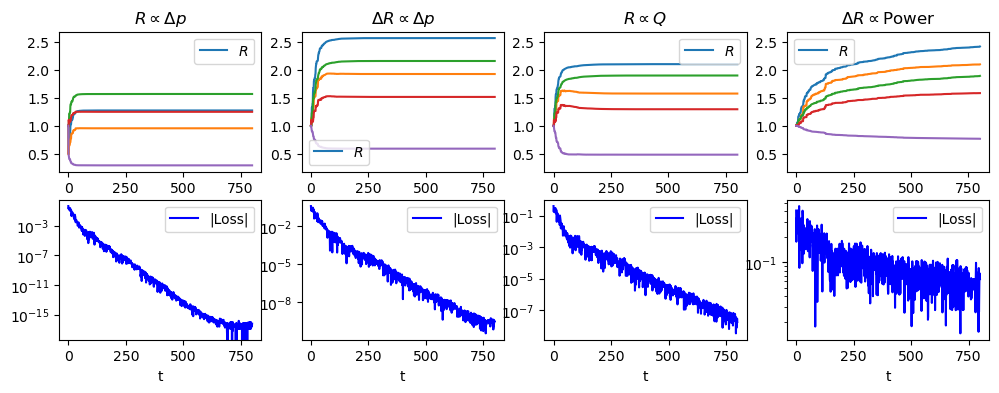
\includegraphics[width=\textwidth,height=\textheight,keepaspectratio]{Figures/different_R_update_schemes.png}
    % }
    % \caption{Resistances $R$ and absolute value of loss as function of training step $t$ for systems with different update rules for resistance, for the same training set. From left to right - $R\propto$ pressure drop on edge, change in $R\propto$ pressure drop on edge, change in $R\propto$ flow velocity through and change in $R\propto$ power dissipation on edge, respectively. In all networks the input samples during measurement were the same. All schemes show an ability to learn under sufficient amount of training steps.
    % \label{fig:different_R_update_schemes}}
    % \end{figure*}
    
    % Even though the resistances of all edges are unity at the beginning of training, the final resistances differ between the cases, so every system finds a different loss minimum in resistance space. This suggests that a vast class of physical networks can be trained to perform regression tasks using the proposed scheme, each possibly learning to perform the task in a different way. \\
    % From here on we show results only for networks whose resistances change as in equation \ref{eq:R_afo_deltap}, while they are still generalizable to other resistance change options. 
    Networks with a simple structure, trained using our scheme, show the ability to learn regression tasks as in equation \ref{eq:task}. The performance for two different regression tasks is shown in figure \ref{fig:variabs_in_t} where the loss decreases and resistances approach steady state values in the course of training. 
    \begin{figure*}[ht]
    \centerline{
    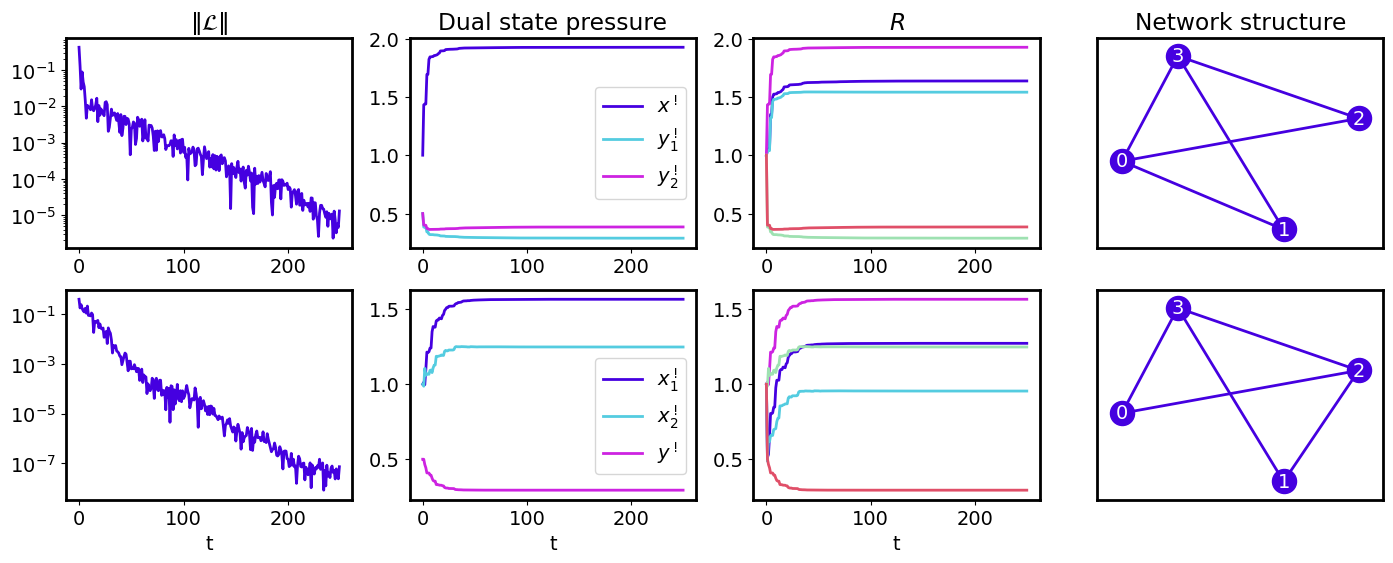
\includegraphics[width=\textwidth,height=\textheight,keepaspectratio]{Figures/performance_2_examples_4panels_mycolors.png}
    }
    \caption{Left to right - absolute value of the loss (normalized by the absolute value of the inputs), the inputs and outputs at the dual state and the resistances as function of training step $t$, and the network structure. Upper panels show the performance of a network with $1$ input, $2$ output and $1$ ground nodes (numbered $0$ to $3$, respectively, in the rightmost panel) trained for the task $y=\left[\begin{array}{cc}0.15 & 0.2\end{array}\right]\left[\begin{array}{c} x_{1}\\x_{2}\end{array}\right]$ and lower panels show a $2$ input $1$ output and $1$ ground nodes network trained for the task $\vec{y}=\left[\begin{array}{c}0.15\\0.2\end{array}\right]\vec{x}$.}
    \label{fig:variabs_in_t}
    \end{figure*}
    The pressure difference between inputs and outputs in the dual state exceeds that in the measured state, so during training, the system is strained beyond the task itself in terms of inputs and outputs. This alludes to an exaggerated directed aging, in contrast to regular directed aging, where a system learns as it is strained to exactly the desired amplitude, and not beyond it.

    The scheme is applicable to tasks of various complexities and is robust to the values chosen for $M$, as shown in figure \ref{fig:log_loss_afo_inputs_outputs}. For specific parameters used in these simulations we refer the reader to appendix \ref{app:net_structure}.
    
    We note that the system exhibits "catastrophic forgetting" (as in \cite{FRENCH1999128} and \cite{stern2020continual}) where training the network successively, task after task, results in the system erasing the memory of previous tasks in place of learning a new one; The system is able to perform only a single task at a time. Nonetheless, a single network can be iteratively trained to execute multiple tasks in sequence, thereby demonstrating the robustness and adaptability of the proposed framework.

\subsection{Scaling up the task}\label{sec:scaling_up}

    As the task complexity grows, i.e. as $M$ grows, the performance decreases, as shown in figure \ref{fig:log_loss_afo_inputs_outputs}. There, even though the number of resistors increases with task complexity, still only tasks with only $1$ input or output can be trained to arbitrarily low loss. This happens because the number of degrees of freedom needed to solve equation \ref{eq:task} is $\left(\# \, \text{Inputs}\times \# \, \text{Outputs}\right)$ whereas the proposed scheme only changes the input and output values in the dual state which are $\left(\# \, \text{Inputs}+\# \, \text{Outputs}\right)$ parameters; The resistances cannot acquire any arbitrary value. \textcolor{roie}{Moreover, it is slightly harder to train a network with many outputs and few inputs than it is the opposite way around, since in the dual state ???.} 
    Nonetheless, to illustrate the success of the proposed scheme in performing regression tasks, albeit the non-vanishing loss at large numbers of inputs and outputs, we compare it to a different, analytical scheme, implemented on our physical system. Here, we aim to analytically find values for the dual state, since they are the degrees of freedom externally controlled by the user. One way of doing so is the following: first, from equations \ref{eq:power_dissipation} and \ref{eq:task} the optimal resistances that perfectly solve the task can be extracted in the form of a sparse matrix $R_{ij}^*$ (here $ij$ denotes an edge connecting node $i$ to node $j$). The pseudo-inverse of the matrix will yield the pressure differences in the dual state $p_i^!-p_j^!=\frac{1}{\gamma}R_{ij}^{*-1}$, that are as close to the sought-after resistances as possible. 
    Nonetheless, this null solution performs worse than a network trained using the proposed training scheme, as shown in figure \ref{fig:pseudo_vs_network_comparison}. 
    We conclude that even though the network performance decreases as the task complexity increases due to limited number of adjustable degrees-of-freedom, it still outperforms non-recursive methods that access the same number of degrees-of-freedom.

    \begin{figure}[ht]
    \centerline{
    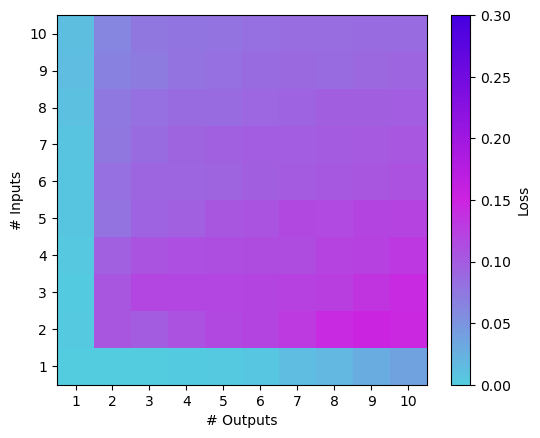
\includegraphics[width=\columnwidth]{Figures/loss_afo_in_out.png}
    }
    \caption{Normalized absolute value of the loss at final training step for tasks with varying number of inputs and outputs, denoted as $\# \, \text{Inputs}$ and $\# \, \text{Outputs}$, respectively. The normalization is with respect to the mean absolute value of the inputs over the whole dataset. Moreover, the figure present the ensemble mean over $8$ runs with randomly chosen $M$, whose entries sum up to $0.5$. The more inputs and outputs there are, the worse the model performs.}
    \label{fig:log_loss_afo_inputs_outputs}
    \end{figure}

    \begin{figure}[ht]
    \centerline{
    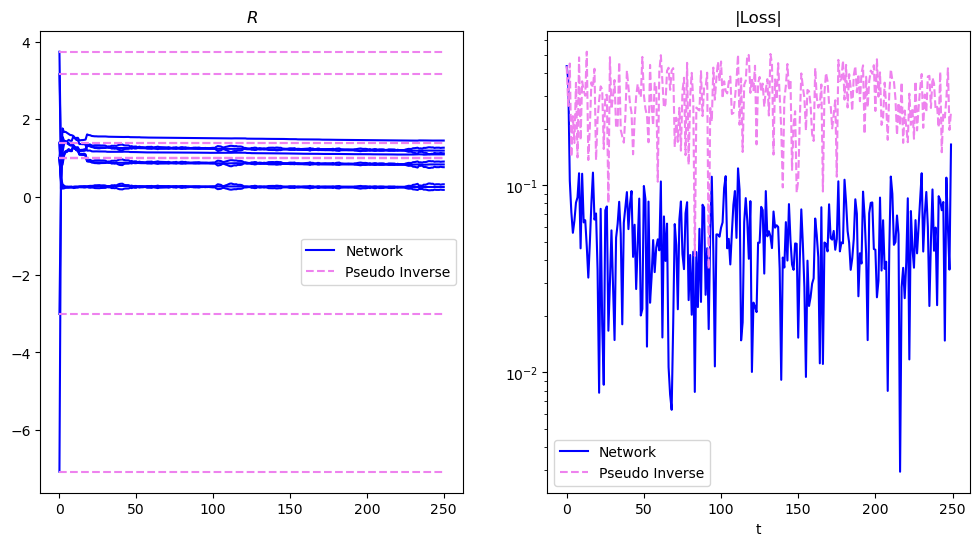
\includegraphics[width=\columnwidth]{Figures/pseudo_vs_network_comparison.png}
    }
    \caption{Comparison between resistances found using the pseudo-inverse and the ones found while training the network for an unsolvable problem of $2\text{ inputs}$ and $3\text{ outputs}$. Left panel - resistances $R$ and right panel - absolute value of the loss, as function of training step $t$. The network performs better than the null guess of the pseudo inverse, even when its resistances are initiated as identical to the ones found using pseudo-inverse.}
    \label{fig:pseudo_vs_network_comparison}
    \end{figure}

\subsection{Classification}\label{sec:Classification}

    Classification tasks are highly non-trivial and are often a staple of versatility and generalizability for learning networks. We tested the performance of the proposed scheme on the iris benchmark dataset \cite{fisher1936use}, where one of three iris species is to be identified using $4$ input parameters. For specific parameters and network structure used we refer to appendix \ref{app:net_structure}. 
    Instead of using a one-hot $3$ dimensional output as desired output for each iris specie, we chose the average output of all samples from the specie. This requires passing all $150$ iris samples in the dataset through the network at the beginning of each epoch and averaging over outputs from all samples of the same specie. Nonetheless, since the network is linear, this averaging is equivalent to passing the average of the inputs of that specie, which simplifies the training procedure; It is essentially tokenizing the outputs to an embedding dimension of $3$, a common practice in training neural networks. We note that the network itself specifies the desired outputs and that these converge to a steady state in the course of training. A correct classification of an iris sample is when the measured output is closest in terms of $L2$ norm to the desired output of that sample. Using our scheme, with a training set of $30$ Iris samples and the remaining $120$ are saved for test, the test accuracym defined as the average of samples correctly classified in the test set, easily reaches $93\%$ after less than an epoch, as in Figure \ref{fig:accuracy_vs_t}. We conclude that our scheme can even perform classification tasks using a linear network.

    \begin{figure}[ht]
    \centerline{
    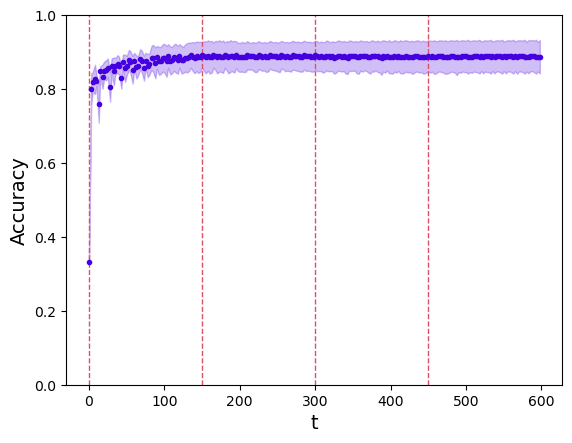
\includegraphics[width=\columnwidth]{Figures/accuracy_vs_t_markers.png}
    }
    \caption{The prediction accuracy as function of training step $t$ (blue), defined as fraction of irises correctly classified from the full iris dataset. Solid line represent the ensemble mean out of $8$ runs and opaque bounds are one standard-deviation from mean. Dashed-red lines mark times when the desired outputs were re-calculated; At the beginning of every epoch, every $150$ training steps.}
    \label{fig:accuracy_vs_t}
    \end{figure} 

\section*{Conclusions}\label{sec:conclusions}

    In this work, we develop a scheme for training a broad class of power-minimizing physical systems to perform a wide range of learning tasks, where the only variables accessible to the user are the inputs and outputs. The scheme capitalizes on some physical law that governs the evolution of the system’s internal degrees of freedom in response to changes in the inputs and outputs. 
    We have shown, by numerical simulations of resistor networks \textcolor{roie}{(and experiment???)}, that these systems can successfully perform a) linear regression and b) classification tasks, similar to a linear artificial neural network. There is, however, a constraint on the regression tasks that can be performed, since the output values of a system that minimizes power dissipation and that has ground nodes are lower than the inputs. Nonetheless, a gain added to the network by way of an amplifier with a learnable amplification amplitude can expand the solvable tasks. The performance is also limited for linear regression tasks in terms of scalability of inputs and outputs, decreasing with increase in the number of inputs and outputs, but nonetheless the network trained using the proposed scheme performs better than a null guess using a determinate pseudo-inverse method. 
    
    The scheme harnesses the advantage of contrastive learning \cite{scellier2017equilibrium} or coupled learning \cite{stern2021supervised} where internal degrees of freedom change due to local rules solely, but differs from it as there is no need for a twin network with constrained outputs or need for storage of the internal state of the whole system during each training step; Our scheme requires memory only of the input and output values. 
    Moreover, the contrastive learning scheme requires measuring a contrast between the internal degrees of freedom in two states, whereas in ours even though the internal degrees of freedom change, there is no need to measure them; They change due to local physical relations and the system learns nonetheless. 
    Physically, in this work the internal degrees of freedom are resistances and the physical relations studied are when resistances are a function of the local pressure drop, current or power dissipation (as presented in section \ref{sec:theoretical}). 
    Figure \ref{fig:accuracy_4_materials} shows that all the above can be trained, affirming that the scheme is applicable to a wide variety of physical materials, i.e. whose resistance responds differently to constraints. While studying the different change rules of resistance, even though the resistances of all edges are unity at the beginning of training, the final resistances differ between the cases, so every system finds a different loss minimum in resistance space. This suggests that each class of materials not only learns to perform the task, but that it does so in a different way.

    \begin{figure}[ht]
    \centerline{
    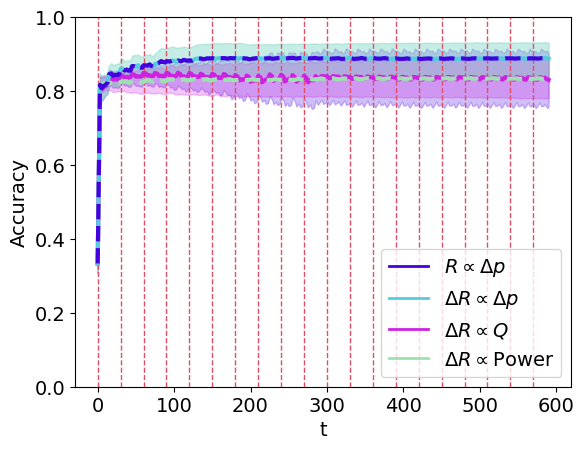
\includegraphics[width=\columnwidth]{Figures/accuracy_vs_t_4_materials.png}
    }
    \caption{Accuracy as function of training step $t$ for the Iris dataset. Here we studied $4$ systems with different change in resistance schemes, relating to $4$ different physical materials: $R_{ij}\left(t\right)=\gamma \Delta p^!_{ij}\left(t\right),\,R_{ij}\left(t\right)=R_{ij}\left(t-1\right) + \gamma \Delta p^!_{ij}\left(t\right),\, R_{ij}\left(t\right)=R_{ij}\left(t-1\right) + \gamma Q^!_{ij}\left(t\right)$ and $R_{ij}\left(t\right)=R_{ij}\left(t-1\right) + \gamma \mathcal{P}^!_{ij}\left(t\right)$. Solid lines represent ensemble averages over $8$ runs and opaque bounds are a standard deviation from mean. dashed horizontal red lines mark times when the desired outputs were re-calculated, i.e. at the beginning of every epoch (every $30$ training steps) while the accuracy was measured every $5$ training steps. All networks show the ability to learn reaching accuracy of above $80\%$, on average, in less than an epoch.}
    \label{fig:accuracy_4_materials}
    \end{figure}
    
    A physical implementation of the scheme could be, for example, an electrical resistor network where resistances increase when the pressure voltage across them grows above a certain threshold. If fluidic networks are sought, pushing a fluid through tubes that clog the more flow goes through them, or that contract due to hydrostatic pressure across them, will also be trainable using our scheme. Similarly, a spring network can be harnessed by way of springs that stiffen the more they are stretched. All of the above are cheap and easily operable, \textcolor{roie}{and we will soon embark on implementing a physical realization ourselves.}\\
    
    On the theoretical level, the learning scheme can be thought of as an exaggerated aging since in order for the system to learn, it has to be strained to values larger than those that perform the task.

    \textcolor{roie}{In regression tasks, the relation to power dissipation is the weakest, do we want to stress that?}


\begin{acknowledgments}
\textcolor{roie}{We wish to acknowledge ???}
\end{acknowledgments}

\appendix

\section{Appendix A - Parameters and network structure}\label{app:net_structure}

For a regression task of $d_{out}$ equations for $d_{in}$ parameters, the structure of all networks is chosen as the following: $d_{in}$ inputs,  $d_{out}$ outputs are fully-connected and each is connected to a single ground node so $d_{in}+d_{out}+1$ nodes and $d_{in}\times d_{out}+d_{in}+d_{out}$ edges (resistors) in total. For the Iris classification task we used networks with $4$ input and $3$ output nodes that are fully-connected, and each is connected to a single ground node. For classification tasks we used a training set of randomly chosen $30$ Iris samples, the remaining $120$ are left for test, under which the test accuracy is measured, and the target outputs are re-calculated as in section \ref{sec:results} every epoch, so every $30$ training steps. In both regression and classification tasks, $\alpha=0.1,\,\gamma=1$ were used.

\nocite{*}
\bibliography{citations}

\end{document}
